
\chapter{Discussion}
\label{chap8}
This chapter will evaluate how the implemented algorithms work, the shortcomings and
possible solutions to problems. 

\section{How did it perform?}
Evaluation of the system is done in this section. The implemented systems are evaluated
and why it did not work as planned are outlined. In the last section
possible changes are proposed that might make the system better. 

The sensors are assessed individually, and then the surface fit algorithms are evaluated.


\subsection{MESA SwissRanger 3000}
The output from the camera was applied directly into Matlab. Default
integration time were used, and the intensity- and range images where captured as is from
the camera electronics.

The normal distributed measurement noise where damped and partly removed by averaging the images over a number
of successive images. This reduced the response time of the sensor and therefor the
refreshment time, but this will most probably not be a case in this application, since the
velocities included are not of the greatest magnitudes. 
The systematic errors described in Chapter \ref{chap2} were difficult to asses just from
looking at the sensor output, but this might be the cause of overestimation of the pipe
radius. 

The field-of-view of the camera is one of its short-comings. In a small confined space
like a pipe environment the field-of-view is important. The full view of the pipe is not 
available at close range to the
robot. This limits the robot to spot obstacles or anomalies along the pipe walls at close
range. The field-of-view of the camera are $47.5^\circ$ in the horizontal directions and
$39.6^\circ$ vertical. This means that if the pipeline is $25$ cm in diameter and the
camera are places exactly in the middle, the full view of the pipe is not available before
\begin{equation}
    \begin{aligned}
        d =& \frac{0.125}{ \tan \frac{47.5}{2}}  = 0.284\\
        h =& \frac{0.125}{\tan \frac{39.6}{2}} = 0.347
    \end{aligned}
\end{equation}
This is 35 cm in front of the robot, which is quite limiting for looking at the pipe walls
up-close, without being able to turn the camera. This is in the ideal case where the
camera is located exactly in
the middle of the pipe. Since most of the obstacles will be on the ground in the pipe it
might be useful to tilt the camera somewhat downwards, to get a better view of the ground
in the front of the robot. 






\subsection{Minoru 3D webcamera}
The stereo camera rig which is used in the project is a cheap mass produced stereo
webcamera. As seen from the calibration in Chapter \ref{chap3} the two different cameras have substantial
distortion, both tangential due to misaligned CCD chip, and radial due to cheap optics.
The CCD chips are horizontally aligned, while in the vertical
direction  are aligned in a divergent way. This will limit the field-of-view of the
camera. The principal axes of the two cameras are unaligned horizontally, which will
further limit the field-of-view. See figures \ref{chap2:fig-tang-dist},
\ref{chap3:fig-comp-lensdist} and \ref{chap8:fig-rad-dist}.
\begin{figure}[htbp]
    \centering
    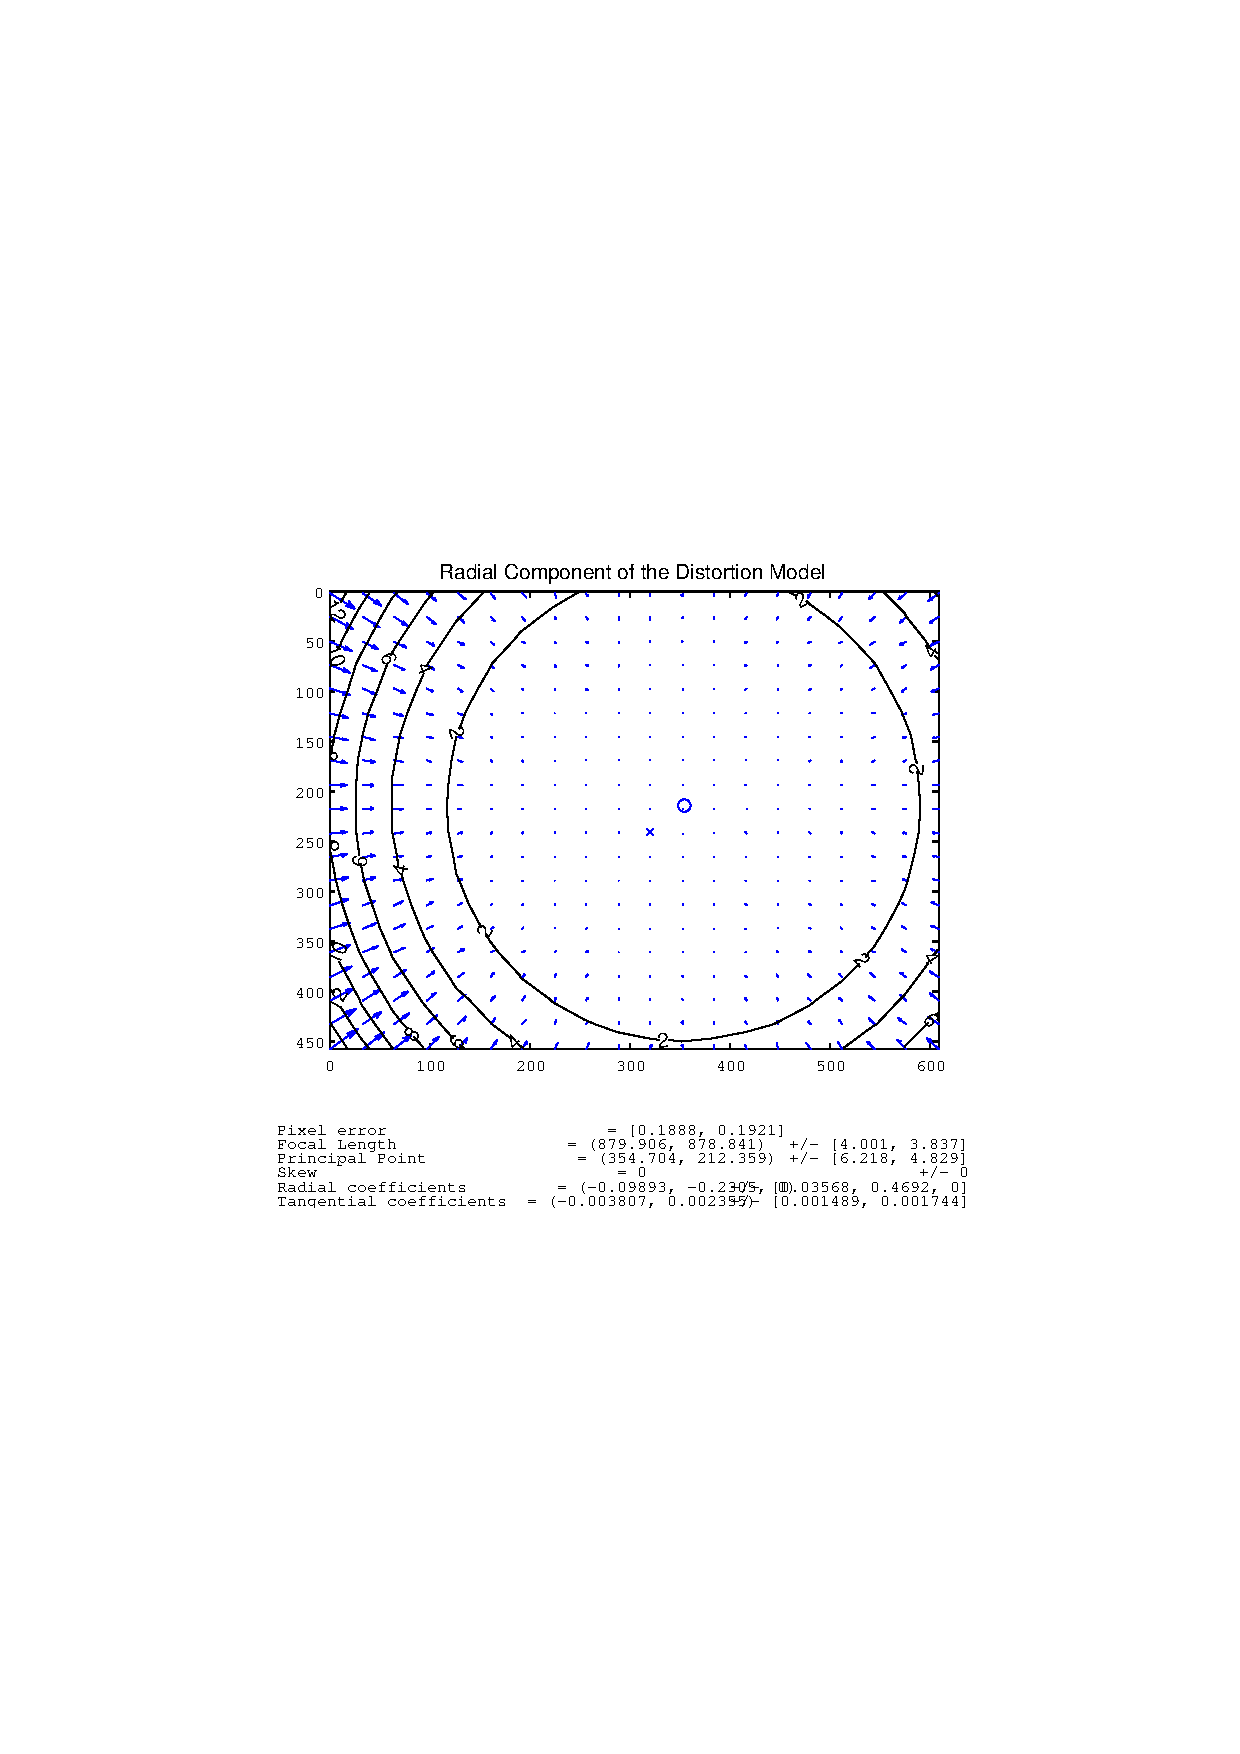
\includegraphics[width=0.45\textwidth]{pics/left_rad_dist}
    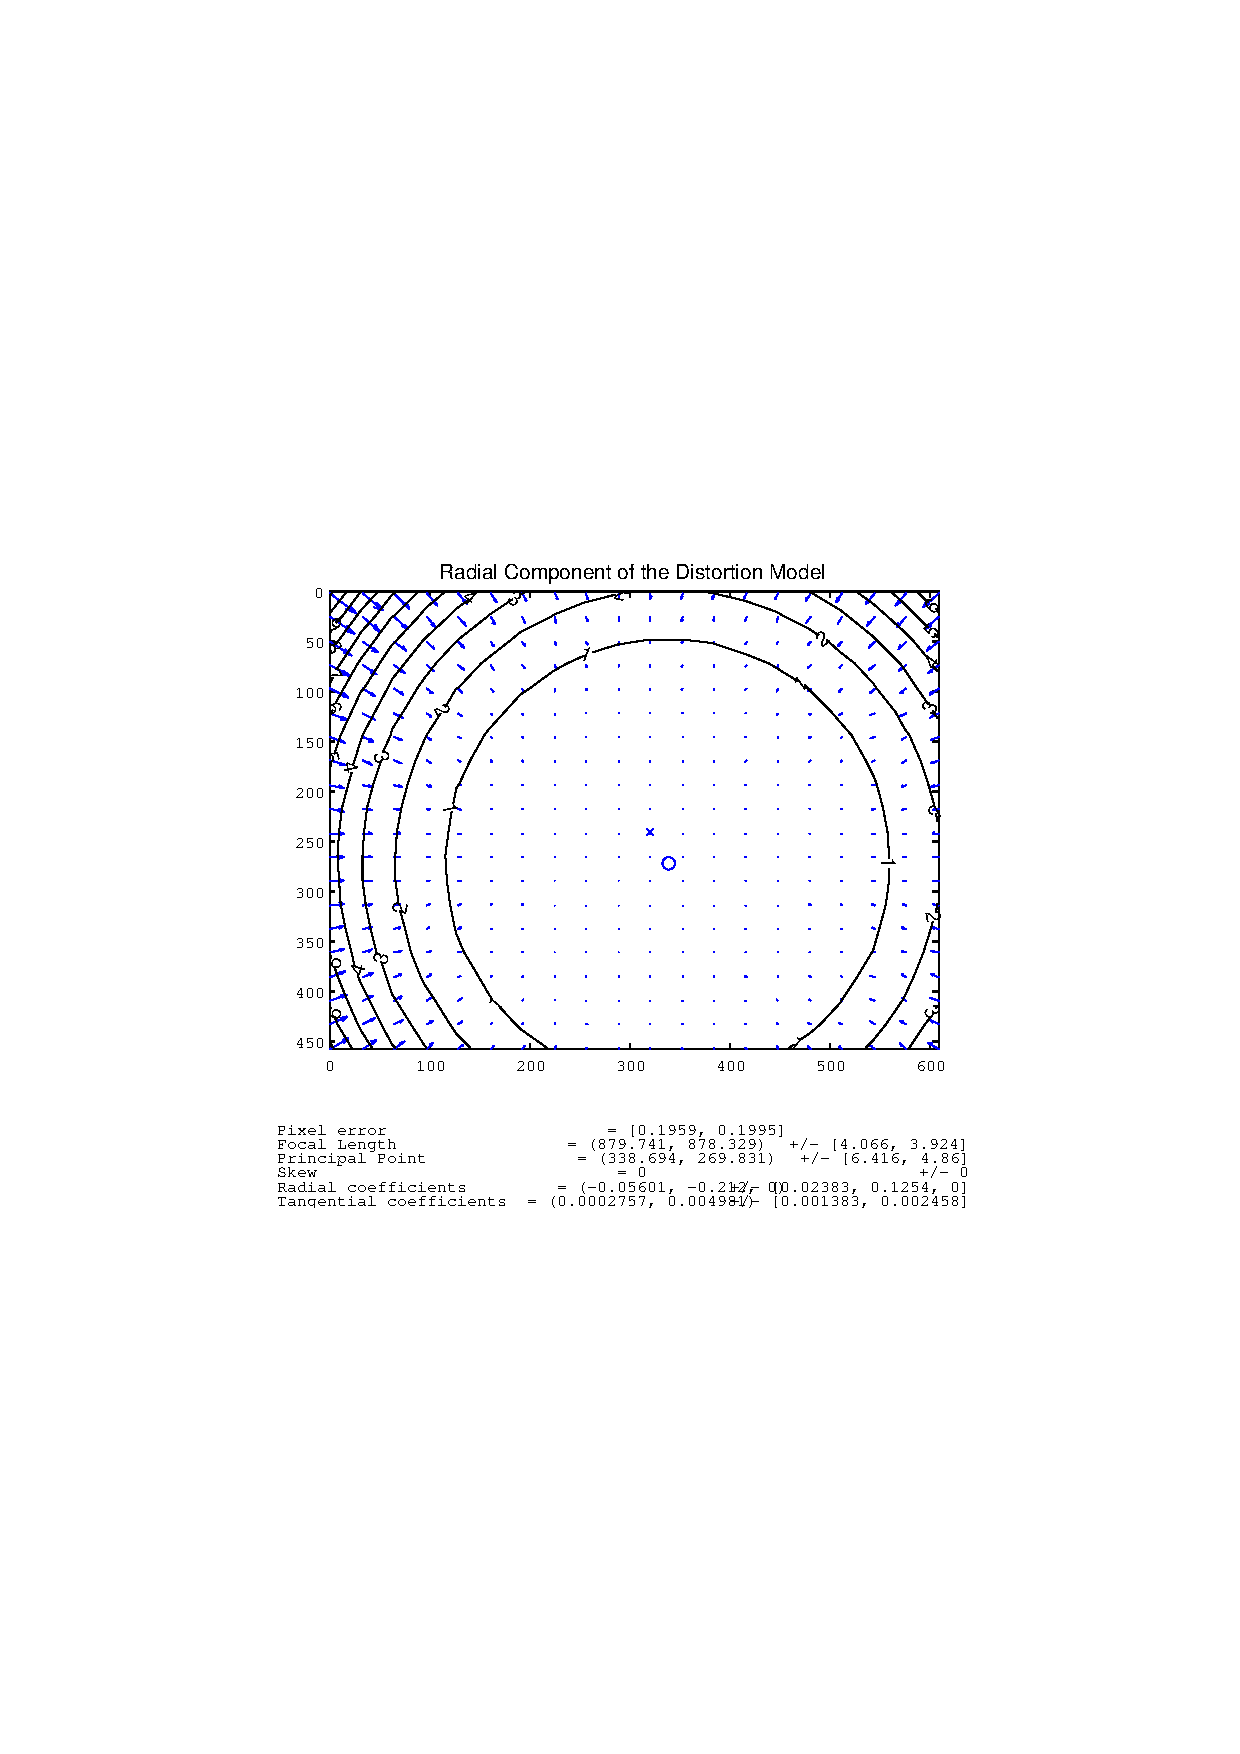
\includegraphics[width=0.45\textwidth]{pics/right_rad_dist}
    \caption{The radial distortions of the left and right camera of the stereo rig}
    \label{chap8:fig-rad-dist}
\end{figure}
The field-of-view of the stereo rig is the incision of the two images. The same arguments
are valid for the stereo cameras as for the time-of-flight camera in the previous section. 

Another limit of the cameras, besides the field-of-view is the light sensitivity and
the amount of noise on the captured images. The amount of noise in the captured pictures
is dependant on the portion of ambient light in the scene. In the tests no extra
light source where used, only ambient light and sunlight. This was because
the pipe bends where turned towards the window which gave much sunlight. An artificial
light source were included in the tests, some of the features would be sharper and the
matching would probably have produced better results, but this might also include problems if the
inside of the pipe are highly reflective, which might cause highlights in the images and 
blend out features. But this might all be used constructively, like \cite{MRINSPECT-V}.
Using shadow profiles to recognize and classify pipeline profiles is an innovative idea,
and might also be used to detect anomalies, such as slag and other obstacles based on the
cast shadows.

The inside of the test pipe were mostly featureless. The implemented algorithms did not
detect enough features in both cameras to calculate a dense stereo image of in most of the
cases. Even when there were obstacles, both irregular and regular objects, the algorithm did not
detect enough features, and where not able to match these features. This might be because
that there were not enough light in the scene and the surfaces of the irregular object
where not sharp enough for the algorithm to detect. Enhancing contrasts and image features
might have given better results, for example using a histogram intensity transform,
although this is done to some extent in the \emph{Open CV} library functions. \cite{gonzalez} 

To test if the algorithm did provide dense stereo images, the stereo rig were directed at
a typical lab environment, with enough structure to make good stereo matches for the
implementation. See figures \ref{chap8:fig-structured-test-rectified} and
\ref{chap8:fig-structured-test-depth}
\begin{figure}[htbp]
    \centering
    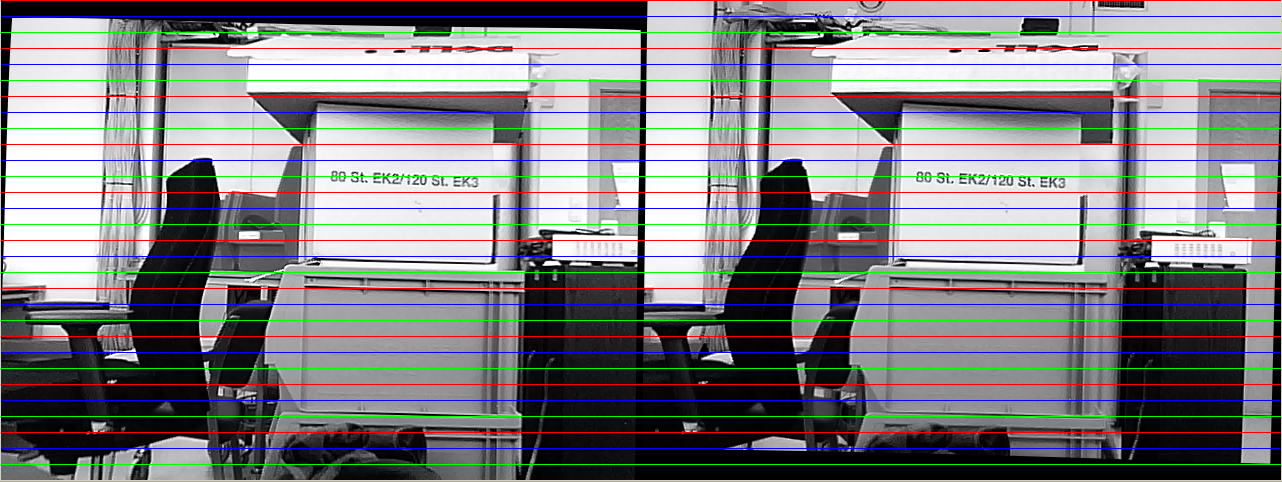
\includegraphics[width=\textwidth]{pics/structure-test-rectified}
    \caption{Rectified left and right images of the structured lab environment}
    \label{chap8:fig-structured-test-rectified}
\end{figure}
The rectified images have the epipolar lines superimposed. The lines can be used to verify
that pixels that are in both images are aligned horizontally.
\begin{figure}[htbp]
    \centering
    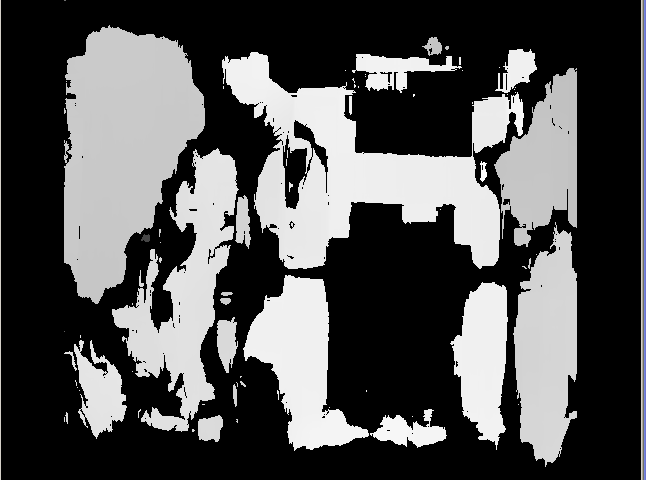
\includegraphics[width=0.35\textwidth]{pics/structure-test-depth}
    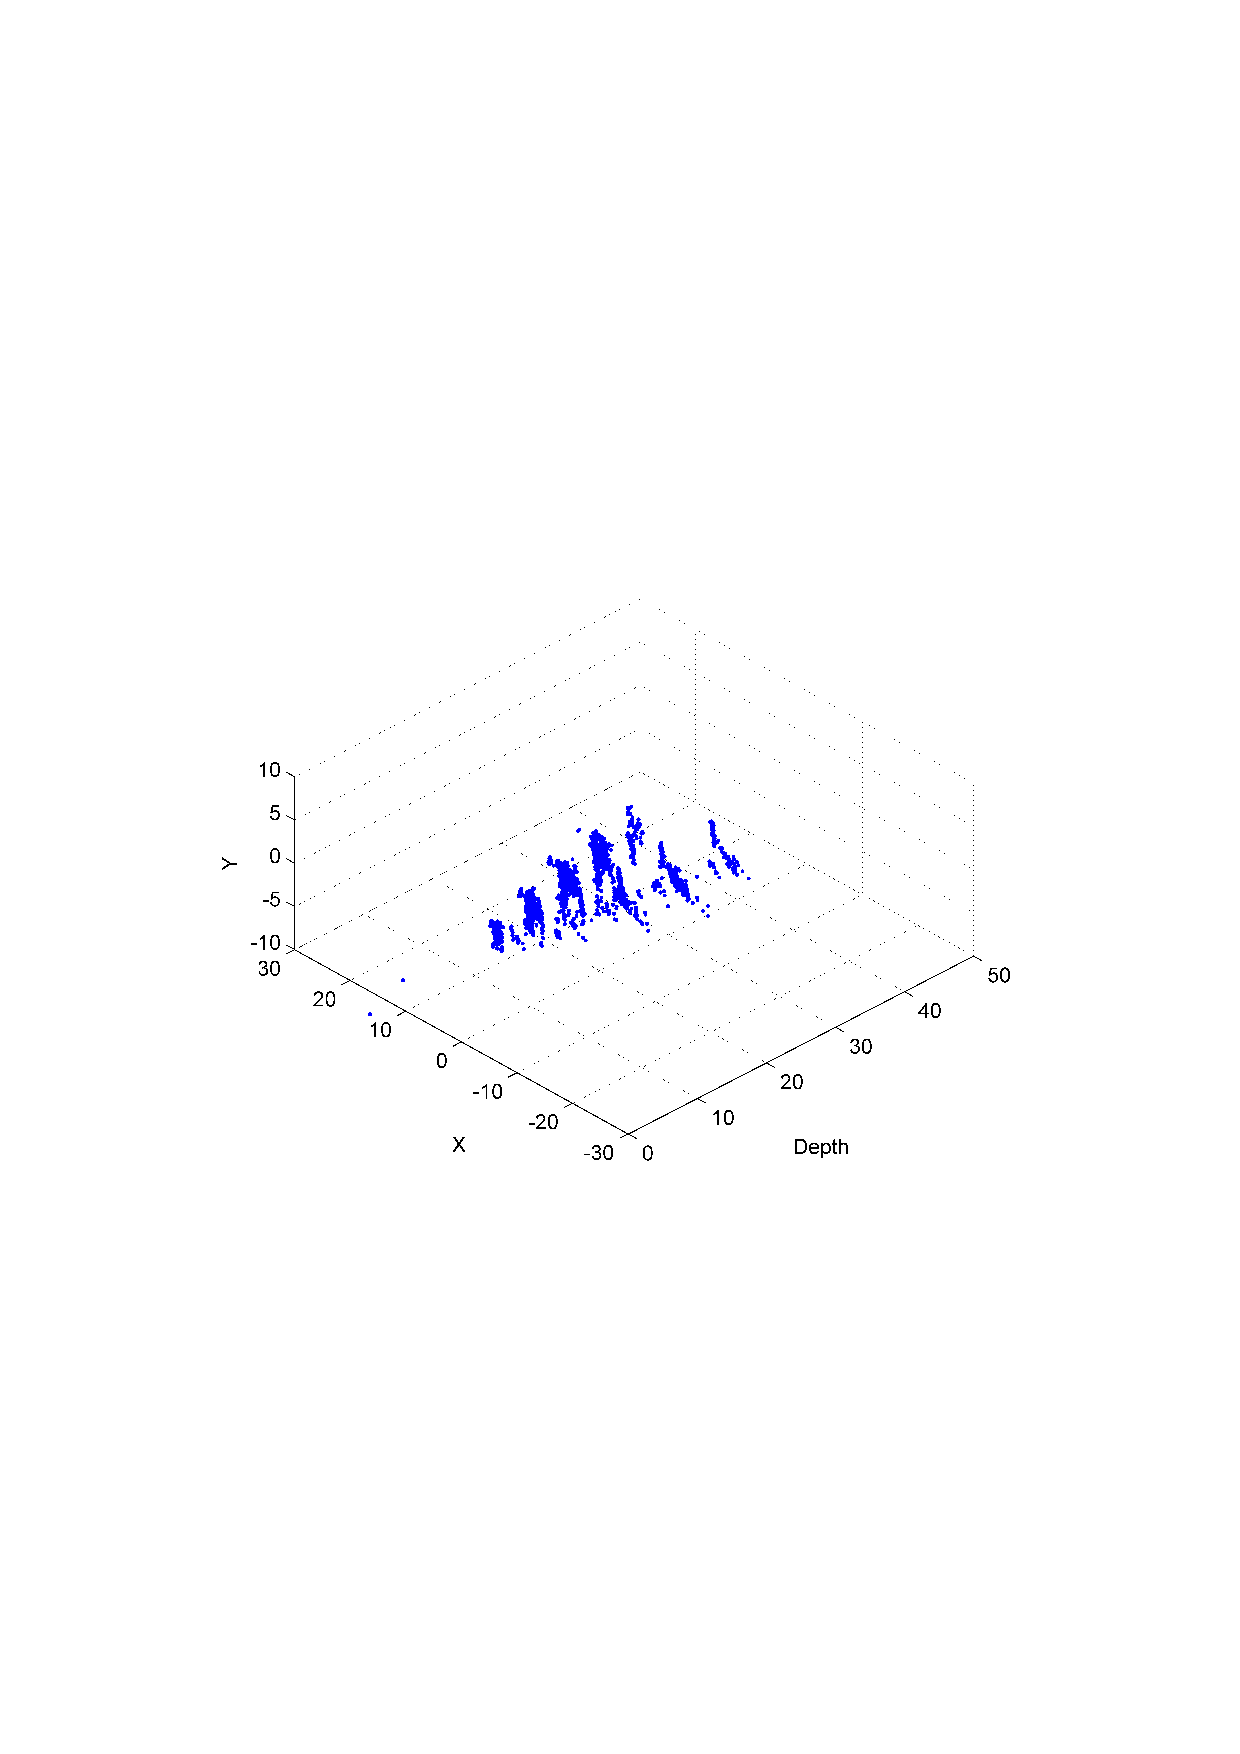
\includegraphics[width=0.55\textwidth]{pics/structured-test3d}
    \caption{Depth image and projected point cloud of the structured lab environment test}
    \label{chap8:fig-structured-test-depth}
\end{figure}
This clearly shows that the rectification and finding stereo correspondences
works adequately for good lit, structured environments. 

The reprojection of the disparity image clearly shows that the object in the
middle is closet to the stereo rig, but the shape of the objects are difficult to make
out. 
The range image is much more detailed than the other reprojected images. This is most probably
because there are sufficient light in the scene and a lot more features which can be
matched.


Another aspect worth noting is when bad matches occur. The figures
\ref{chap8:fig-pos21-control-depth} and \ref{chap8:fig-pos21-control-rectified} show an
example of this. The periodic structure on the walls in the pipe bend is the problem. The
distance from the wall makes the structures fall almost exactly on top of each other,
but the structure is shifted one of the structure length to the left. This makes the
disparity of the two features small, which means that the distance must be far away. 
\begin{figure}[htbp]
    \centering
    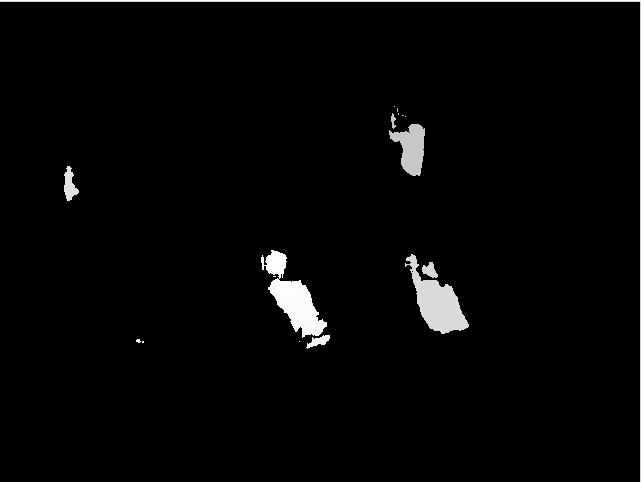
\includegraphics[width=0.35\textwidth]{pics/pos21-control-depth}
    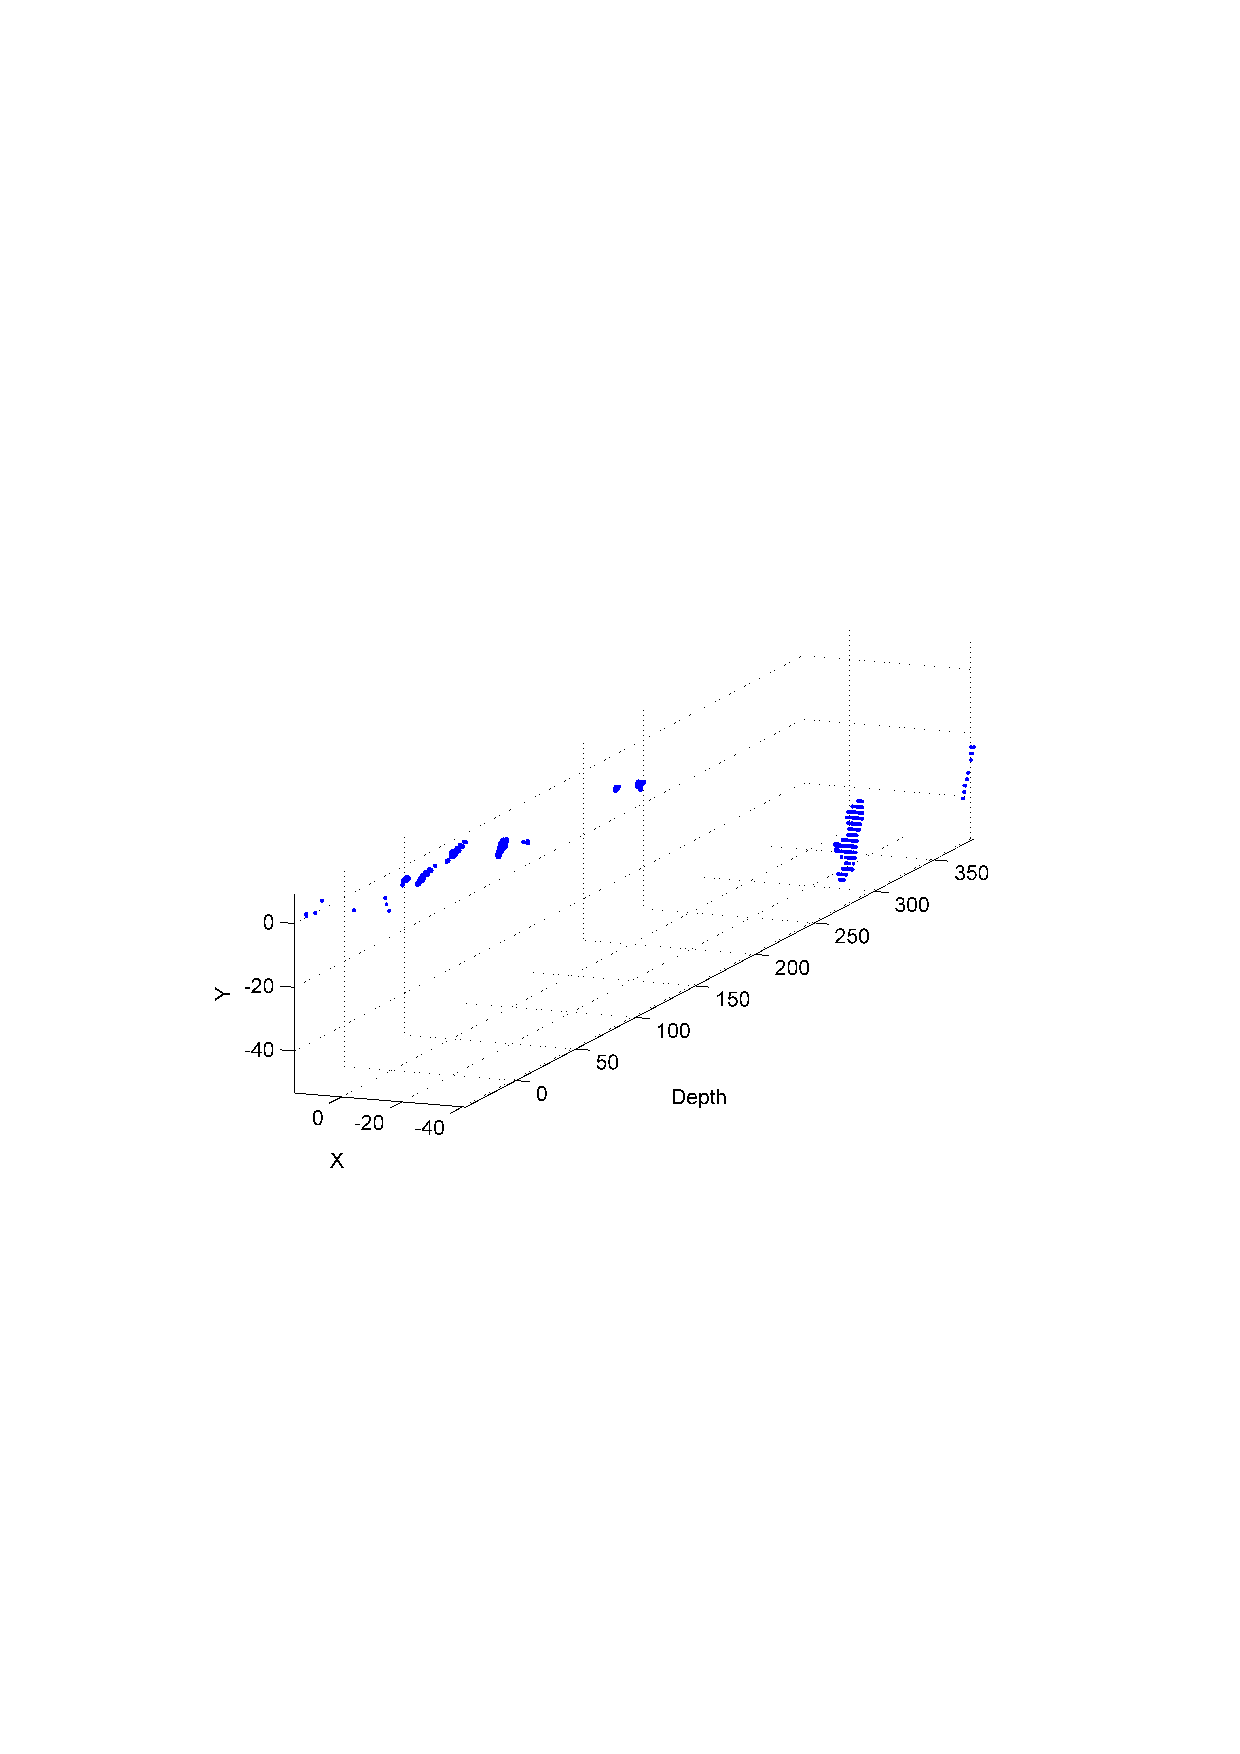
\includegraphics[width=0.55\textwidth]{pics/pos21-control-3d}
    \caption{Depth image and projected point cloud of the structured lab environment test}
    \label{chap8:fig-pos21-control-depth}
\end{figure}
\begin{figure}[htbp]
    \centering
    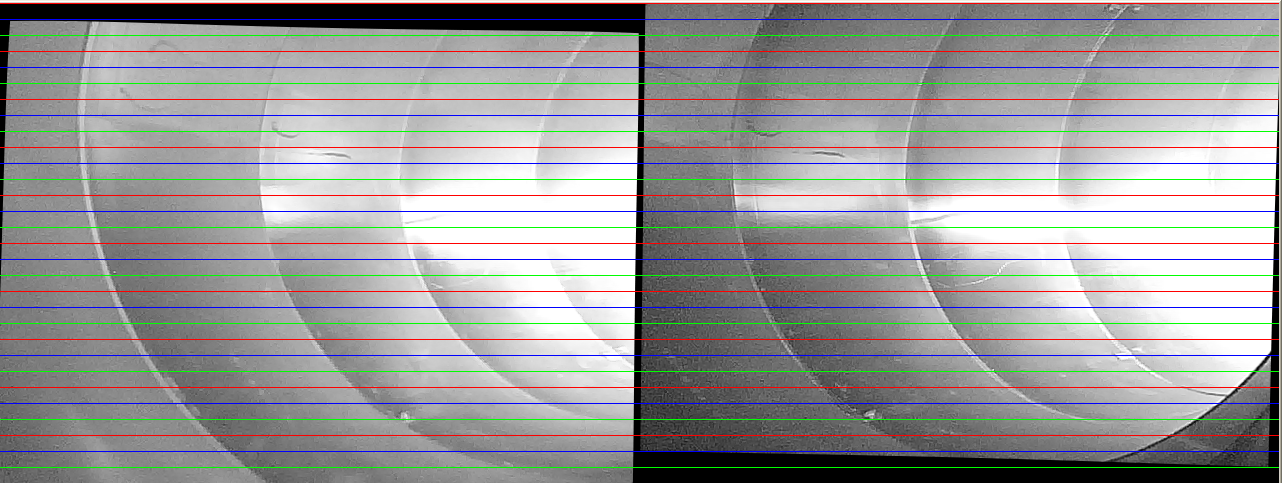
\includegraphics[width=\textwidth]{pics/pos21-control-rectified}
    \caption{Stereo Pair of the bad matches}
    \label{chap8:fig-pos21-control-rectified}
\end{figure}
This is exactly what is shown in the right plot in Figure
\ref{chap8:fig-pos21-control-depth}. The distance to the matched points are calculated to
be very far from the view, because of the small disparity. This is the danger when the
environment is periodically structured, and at given distances this can happen.
Projecting structured light on the environments is a way of helping the matching procedure
in environments with little structure, and might have given better results in this case. 

When regarding speed, the \emph{OpenCV} library is reasonably fast. When running at
$640\times480$ a brute-force implementation of the stereo matching using standard
\emph{OpenCV}-library methods, where able to process 2-3 stereo pairs, and
output a dense stereo range image, each second on a Pentium 4 3.0 GHz Windows XP 
standard workstation with 2 Gb of RAM. 

The last question is how can this be implemented on an embedded platform, which has limited
computational abilities? Porting the \emph{Open CV} library to an embedded platform is a
topic that is not much discussed, and is probably more work than the gain. The solution
here is most probably to implement this stereo matching algorithm that is highly optimized
for the implementation platform. 




\subsection{Hokuyo URG-04LX Laser Range Finder}
The measurement errors from the laser range finder that affects the readings in the test were
mostly random Gaussian distributed noise. To get rid of this, 5 successive
readings where averaged. Since the update rate of the range finder is 10 Hz, the system
will get readings from the URG twice every second. This will not impact the control system
that much, since the dynamics of the system is not that fast. The implementation, the time
needed to get a full range scan was about 0.1-0.15 seconds. The times seemed a bit random,
and where dependant on the time to locate enough memory to store the scan. 

The range finder gives dense data near the position of the sensor, and more sparse data
when far away, which is obvious because of the nature of the scanning. The scanner does
also have a large field-of-view that makes it a good addition to the sensor suit of the
platform. 

The sensor is limited to planar measurement. Depending on the position of the laser
scanner, this will limit the ability to sense obstacles which does not cover a large part 
of the pipe. Obstacles in a pipe environment might be sediments and residues of the medium
travelling in the pipe, and they usually settle at the bottom of the pipe. If the range
finder is placed high above the ground in the pipe, these sediments and potential
obstacles will not be detected. This motivates the use of the sensor for estimating the
pipe radius and matching profiles, since in many cases the obstacles in the pipe will not
affect the pipe profile, seen from the range finder. 


\subsection{Surface Fit and Pipe Properties Estimation}
The proposed surface fit algorithm is based on the least-squares method. This does not
work very well 
when there is no segmentation employed in the system. Looking at Figure
\ref{chap7:fig-longpipe-tof-3d} from the Long pipe test, the first cylinder axis is severely displaced. This
is because of pipeline profile. The Y-junction is recognized as half a cylinder. The
other cylinders are however fitted better to the point cloud. Although the axis are 
directed somewhat upwards. The direction vectors are given below in Equation
\eqref{chap8:eq-direction-longpipe}. This might have something to do with the pose and
alignment of the Time-of-Flight camera when capturing the snapshot.
\begin{equation}
    \label{chap8:eq-direction-longpipe}
    a_1 = \left[ \begin{matrix}
                        0.8165\\
                       -0.1749\\
                       0.5503 
                 \end{matrix} \right] \quad a_2 = \left [
                 \begin{matrix}
                       0.0009\\
                       0.08657\\
                       0.9963
                 \end{matrix} \right] \quad a_3 = \left [
                 \begin{matrix}
                       -0.0997\\
                       0.1185\\
                       0.9879
                 \end{matrix} \right]
\end{equation}
Vector $a_2$ and $a_3$ are almost parallel with the $z$-axis, which is the view direction,
and also the direction of the pipe. But the axes are offset in the $y$-direction which tilts
the cylinder axis upwards. This might all be due to the sensor not placed entirely with
the principal axis horizontal. 

Figure \ref{chap7:fig-longpipe-tof-dist} is a measure on how good the cylinder fits. The
figure has small crosses where the next cylinder interval starts. The $x$-axis show
the number of points which is fitted to the cylinder and the $y$-axis scale is in meters.
As seen from the figure, the overall distance of the points to the given cylinders is in
general less than 5 cm, this is not a great result, but it suffices and gives the general
direction of the pipe. This collection of points might be used for a crude selection
criterion for which point indices that might belong to the cylinder. The algorithm might
then be run once more on the filtered point selection, and give a better cylinder fit to
selected set. 

For the laser range finder data, the line fitting worked quite well, see
Figure \ref{chap7:fig-longpipe-urg-2d}. For the horizontal lines, the walls of the pipe
are detected adequately. The errors for the fitted horizontal lines are oscillating
around zero, except for the ends of the lines. The vertical line fit , which
really is transversal lines in the plane, are another story. The histogram bins for the
vertical lines where chosen large in this test, and this can be seen because all the lines
which really should have been vertical on the figure are either drawn to the left or right
of the vertical axis, but this lines are of less importance. 


\begin{figure}[htbp]
    \centering
    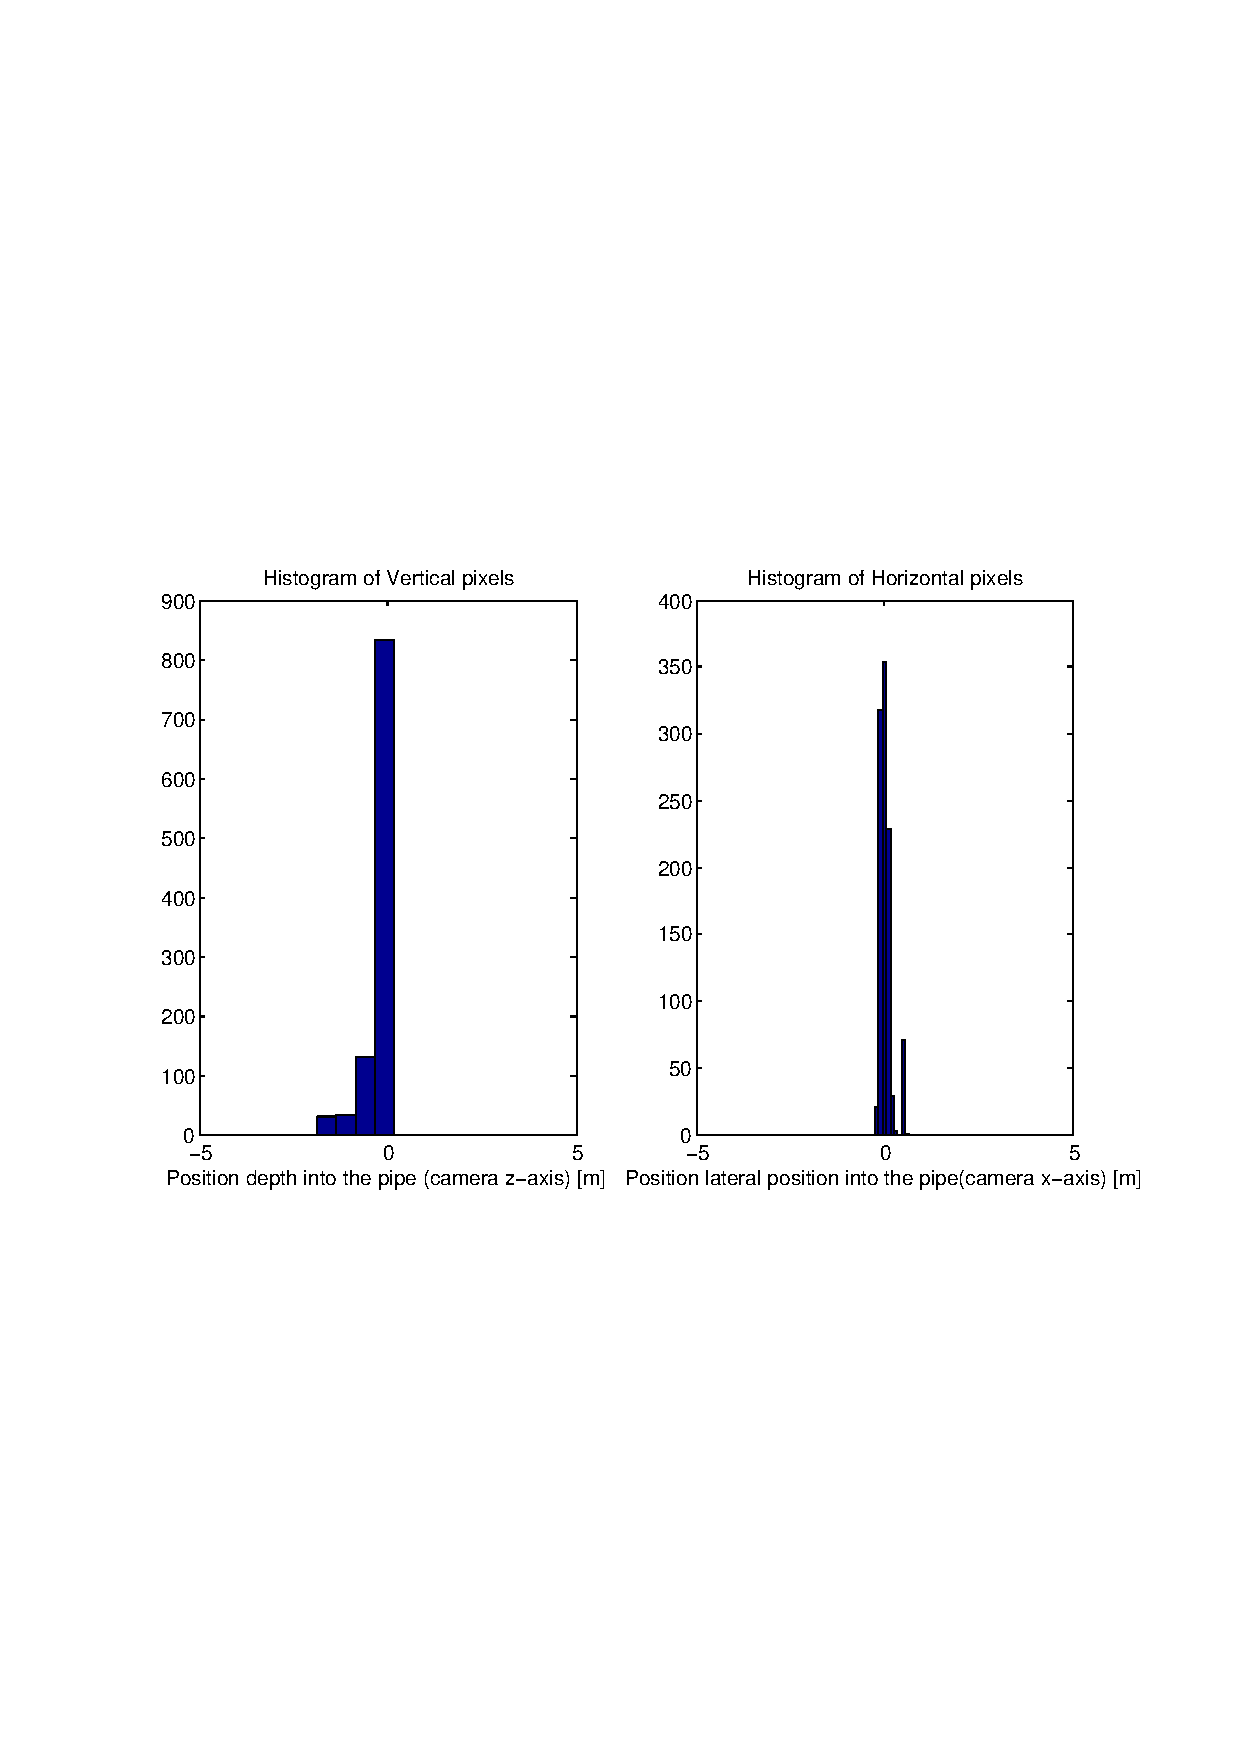
\includegraphics[width=0.9\textwidth]{pics/longpipe-urg-hist}
    \caption{The histogram for the vertical and horizontal line fit for the long pipe test}
    \label{chap8:fig-longpipe-urg-hist}
\end{figure}
Figure \ref{chap8:fig-longpipe-urg-hist} shows the distribution of the points in the
histogram bins. As seen, there are most points in the bin containing the trivial points; this is
because of the sectors of the laser range finder which cannot be measured. These points are
not removed from the data set, but not included in the line fitting algorithm. 
The second plot in the figure clearly shows that there are three distinct gathering of
points with almost the same y-coordinates, which makes up the three walls of as seen on
Figure \ref{chap7:fig-longpipe-urg-2d}. Two walls of the pipe, the third is the window
pane outside the pipe. 

When estimating the radius of the pipe based solely on the laser range finder, the
following result is produced. 
\begin{figure}[htbp]
    \centering
    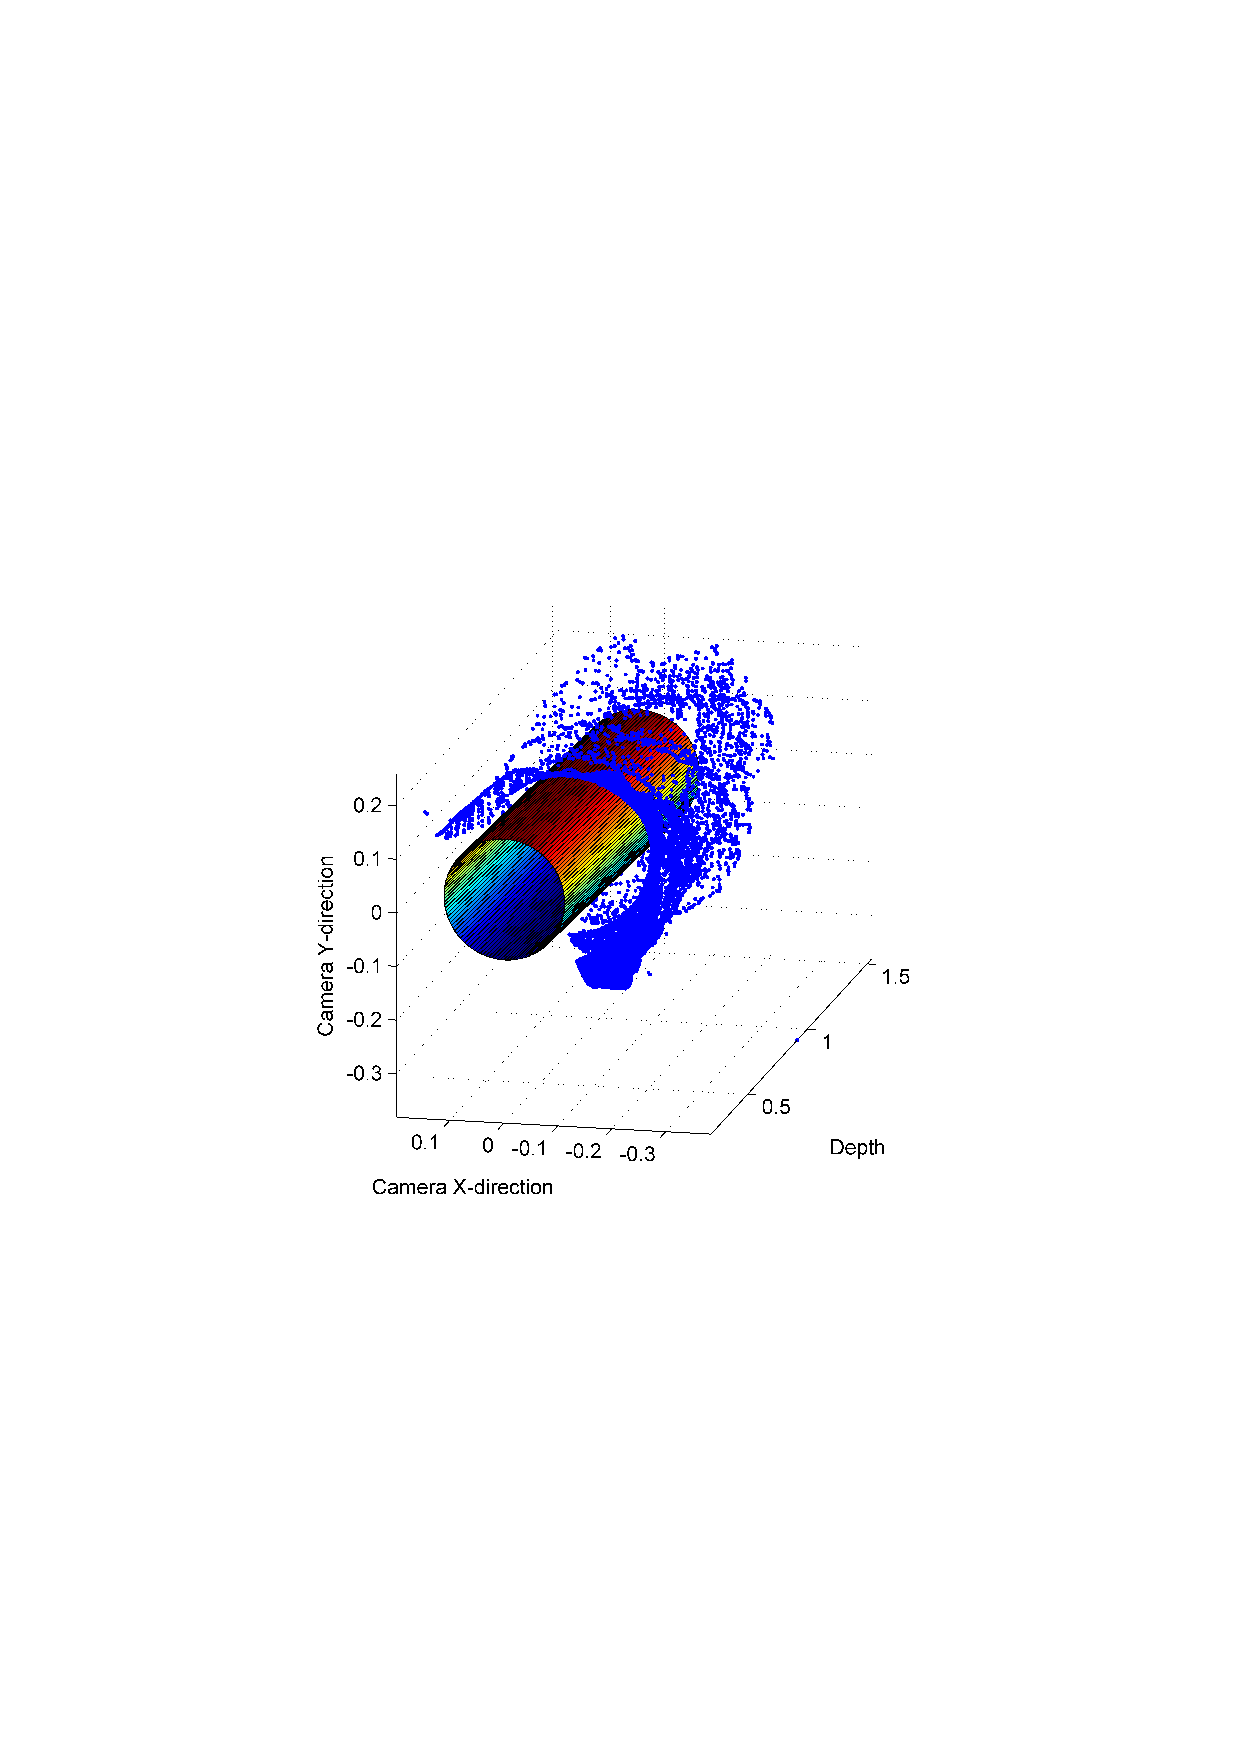
\includegraphics[width=0.8\textwidth]{pics/longpipe-urg-3d}
    \caption{Estimated cylinder using data from Laser Range Finder}
    \label{chap8:fig-longpipe-urg-3d}
\end{figure}
The cylinder is fitted right in the middle of the point cloud. The radius is calculated to be $r = 0.1125$. This
is 1 cm smaller than the actual radius of $r_r = 0.1225$. This difference is most
probably because the hight of the measurement plane was not recorded exactly, and therefor
underestimating the radius. 

When this is shown together with the point cloud, it is
possible that the time-of-flight camera have overestimated the distances at close range,
and therefor making the cylinder appear larger than it really is. 

\cite{sintef-tof} found
that the measurements would narrow as the range increased. Because of this the authors
found that using a cone, gave better fit to the dataset, and gave a better
estimate of the direction and radius. 


When looking at the tests with irregular objects, and looking at the fitted cylinder of
the test at position 1, shown in Figure \ref{chap7:fig-pos1-irregular-tof-3d}, the
cylinders are totally off axis, while the estimated cylinder from the range finer
estimates correct, Figure \ref{chap7:fig-pos1-regular-urg-3d}. This is of course again
because there is no segmentation of the objects in the images, which caused the cylinder
fit to fail in most of the cases. 

With the stereo rig, it was not possible to obtain dense enough point clouds for the
cylinder fit. The algorithm did not converge in all cases. 

\section{Possible Changes}
What could make the system better? In retrospect, after tested the system, it would
benefit from a better feature and estimation scheme. The RANSAC algorithm has proven
efficient in computer vision applications, because of its internal segmenting of points in 
the dataset. This will probably give good results with ``flying points'' that does not
belong to the geometrical primitive. 

Another approach is to use point feature histograms to segment the dataset and separate it
into geometric primitives, which then can be estimated using the fitting algorithms or a
fingerprint of the dataset can be generated and matched to a database, containing
different junctions and features which the robot might encounter. 

A stereo rig provides acceptable results at transitions in the environment, i.e. edges and
structures, while the time-of-flight camera seems to have more problems at these locations.
Therefor a fusion of these sensors might prove useful to avoid, flying pixels and give good
range estimates at edges. \cite{tof-stereo-fusion} shows promising results using this
approach. 

To get better results from the stereo rig, better cameras and light would help. Also using
structured light, such as a laser light pattern projected on the pipeline walls and
recognizing the distortion of the pattern, would give denser stereo information in little
structured environments. Later versions of \cite{makro-plus} use this scheme with promising
results. 


